\documentclass[12pt, letterpaper]{article}
\usepackage[utf8]{inputenc}
\usepackage{indentfirst}
\usepackage{graphicx}
\usepackage{setspace}
\usepackage[numbers]{natbib}
\usepackage [autostyle, english = american]{csquotes}
\MakeOuterQuote{"}
\usepackage{layout}
\usepackage[title]{appendix}
\usepackage[justification=centering]{caption}
\usepackage{titlesec}
\usepackage[percent]{overpic}
\usepackage{amsmath}
\usepackage{systeme}
\usepackage{blkarray, bigstrut}
\usepackage{tikz}
\usetikzlibrary{tikzmark}
\usepackage[utf8]{inputenc}
\usepackage{relsize}
\usepackage[nameinlink, capitalize, noabbrev]{cleveref}
\usepackage{tabu}

\setlength\parskip{\baselineskip}

%prevent hyphenation of words
\emergencystretch=\maxdimen
\hyphenpenalty=10000
\hbadness=10000

\begin{document}

\setcounter{secnumdepth}{-1}
\titlespacing*{\section}{0pt}{1.5\baselineskip}{.25\baselineskip}
\binoppenalty=\maxdimen
\relpenalty=\maxdimen

\setlength{\abovedisplayskip}{-0.5\baselineskip}
\setlength{\belowdisplayskip}{0\baselineskip}
\setlength{\abovedisplayshortskip}{0\baselineskip}
\setlength{\belowdisplayshortskip}{0\baselineskip}

%Cover page: 5pts
%Course, subject, name, date
\title{MA348 Numerical Analysis, Function Interpolation}
\author{David Jefts}
\date{April 8\textsuperscript{th}, 2019}
\begin{titlepage}
	\centering
	\maketitle
	\centering
	\hfill
	\vfill
	\thispagestyle{empty}
\end{titlepage}

\setlength{\voffset}{-0.5in}
\setlength{\headsep}{10pt}

%Introduction: 5pts
%Describe the problem and state objectives
\section{\label{sec:intro}Introduction}
	%Use both the Newton divided differences polynomial and the Lagrange polynomial to approximate ln(2) given the following points: ( you will use polynomial of degree3)
	The purpose of this lab is to use Newton's Divided Difference Polynomials and Lagrange Polynomials to estimate the value of a function at any given point, using only a set of $x-$ and $y-$values. The function to be estimated is the natural logarithm function at the point $x=2$ ($ln(2)$). The estimated line was drawn with the following points:
		
	\begin{align*}
		x && y \\
		(1, && 0.0) \\
		(4, && 1.386294) \\
		(5, && 1.609438) \\
		(6, && 1.791759) \\
	\end{align*}
	
	The Lagrange Polynomial portion of this lab is based on the fact that interpolating a line through four distinct points requires a minimum polynomial degree of three.

%Theory-Analysis: 5pts
%State assumptions and develop equations
\section{\label{sec:theory}Theory-Analysis}
	 Newton's Divided Differences Interpolation Polynomial is a polynomial used to estimate the value of a function when the exact function and its line are not known. This lab was based on creating a polynomial of degree three using four distinct points. The Interpolation Polynomial combines a series of successive Newton Differences into a polynomial using the formula:
	 
	 \begin{equation}N(x)=[y_0]+[y_0, y_1](x-x_0)+\ldots+[y_0, \ldots, y_k](x-x_0)(x-x_1)\ldots(x-x_k)\end{equation}
	 
	 The bracketed $y$ values ($[y_0]$, $[y_0, y_1]$, etc.) are Newton Divided Differences of varying sizes based on the following formula:
	 
	 \begin{align*}
	 	\text{Degree one: } && [y_0] = & f(x_0) \\
		\text{Degree two: } && [y_0, y_1] = & \frac{[y_1]-[y_0]}{x_1-x_0} = \frac{f(x_1)-f(x_0)}{x_1-x_0} \\
		\text{Degree three: } && [y_0, y_1, y_2] = & \frac{[y_1, y_2] - [y_0, y_1]}{x_2-x_0} = \frac{\frac{f(x_2)-f(x_1)}{x_2-x_1} - \frac{f(x_1)-f(x_0)}{x_1-x_0}}{x_2-x_0} \\
	\end{align*}
	
	There were no assumptions made in this lab.

	 
%Numerical Solution: 20pts
%Describe the numerical methods used to solve the problem
\section{\label{solution}Numerical Solution}
	The entirety of the Newton Divided Differences interpolation method was coded in Python, with the report created in \LaTeX{}.
	
	The divided differences are based on finding derivates, which are used to draw a slope between two points. Usually they are depicted in a table, since each successive divided difference uses the divided differences from the previous iteration and the next point like so (where \{DD $n$\} stands for divided difference of degree $n$):
	
	\begin{table}[h]
	\centering
	\begin{tabular}{>{$}c<{$} >{$}c<{$} >{$}c<{$} >{$}c<{$}}
	x \text{ input} & \text{DD 1} & \text{DD 2} & \text{DD 3} \\
	x_0 & f(x_0) &&  \\
	&& \frac{f(x_1)-f(x_0)}{x_1-x_0} & \\
	x_1 & f(x_1) && \frac{\frac{f(x_2)-f(x_1)}{x_2-x_1} - \frac{f(x_1)-f(x_0)}{x_1-x_0}}{x_2-x_0} \\
	&& \frac{f(x_2)-f(x_1)}{x_2-x_1} & \\
	x_2 & f(x_2) && \frac{\frac{f(x_3)-f(x_2)}{x_3-x_2} - \frac{f(x_2)-f(x_1)}{x_2-x_1}}{x_3-x_1} \\
	&& \frac{f(x_3)-f(x_2)}{x_3-x_2} & \\
	\vdots & \vdots &  & \vdots \\
	 &  & \vdots &  \\
	\vdots & \vdots &  & \vdots \\
	x_n & f(x_n) &  &  \\
	\end{tabular}
	\end{table}
	
	The highest entry in each column is then used as the coefficient of the interpolation polynomial. Each coefficient is multiplied by $(x-x_i)$ $(k-1)$ number of times with the following formula:
	
	\begin{equation*} \begin{split}
	N(x) = \text{DD1} + \text{DD2}(x-x_0) + \text{DD3} (x-x_0)(x-x_1) + \text{DD4} (x-x_0)(x-x_1)(x-x_2)
	\end{split} \end{equation*}
	
	Once the polynomial is created, it can be used as a function to estimate the value of any point on the interpolated function line.


%Results and Discussion: 45pts
%Tabulate and plot the results, compare results, and discuss the accuracy of results
\section{\label{sec:results}Results and Discussion}
    	The table of the divided differences values and coefficients (rounded to four decimal places) as described in the Numerical Solution Section is shown below:
	
	\begin{table}[h]
	\centering
	\begin{tabular}{>{$}c<{$} >{$}c<{$} >{$}c<{$} >{$}c<{$} >{$}c<{$}}
	x \text{ input} & \text{DD 1} & \text{DD 2} & \text{DD 3} & \text{DD 4}\\
	1.0 & 0.0 &&&  \\
	&& [y_0, y_1]=0.4621 && \\
	4.0 & 1.3863 && [y_0, y_1, y_2]=-0.1969 \\
	&& [y_1, y_2]=-0.3254 & & [y_0, y_1, y_2, y_3]=0.1450 \\
	5.0 & 1.0609 && [y_0, y_1, y_2]=0.5281 \\
	&& [y_2, y_3]=0.7308 && \\
	6.0 & 1.7918 &  &  \\
	\end{tabular}
	\end{table}
	
	The final polynomial is therefore:
	
	\begin{equation*}
	f(x) = 0.4102249 + 0.3285789(x-1.0) + 0.0189155(x-1.0)(x-4.0) + 0.0078654(x-1.0)(x-4.0)(x-5.0)
	\end{equation*}
	
	Simplified:
	
	\begin{equation*}
	f(x) = 0.0078654x^3 - 0.0597385x^2 + 0.462098x + 0
	\end{equation*}
	%$(C)x^3+(-B-10C)x^2+(A+5B+29C)x+(-A+4B-20C)$
	\newpage
	Below is the graph of the interpolated polynomial, the initial input coordinates, and the estimated value for ln(2):
	\begin{figure}[htp]
            			\centering
            			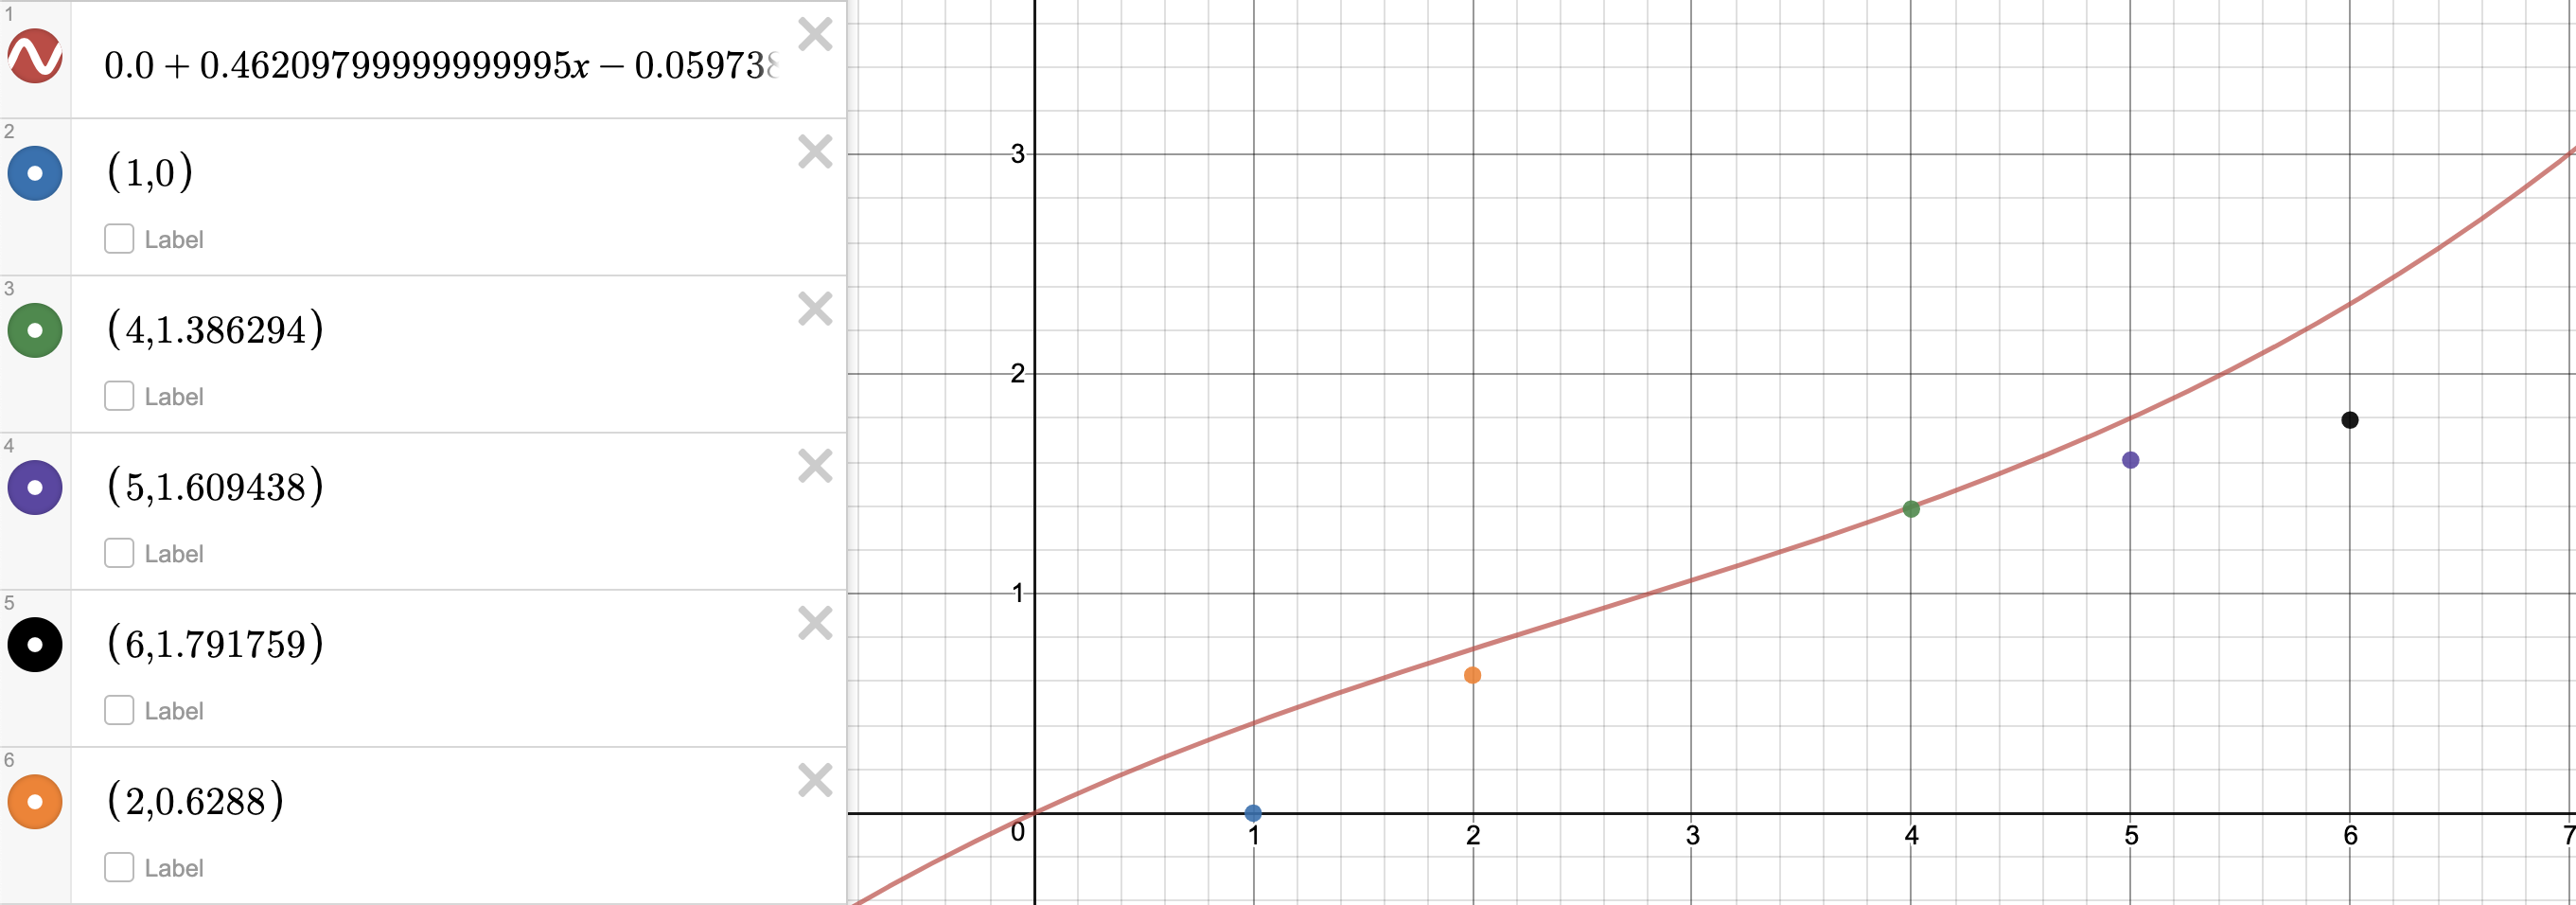
\includegraphics[width=1.0\linewidth]{plot.png}
            		\end{figure}
	


%Conclusions: 20pts
%Comment on the efficiency of the solvers
\section{\label{conclusion}Conclusions}
	The Newton Divided Differences method is very effective at interpolating functions from a set of points, however the results from this lab may have been much more accurate with the utilization of more input coordinates. Additionally, this method seems to require a degree of precision not always possible with some modern calculators and computers. In conclusion, the Newton Divided Differences Interpolation Method is effective at estimating function. curves, but it requires a significant amount of points to increase its accuracy. 

\pagebreak
%Appendices
%Include listings of the source codes, include printed copies of the output files
\appendix
	\section{Appendix A}
            	\begin{figure}[h]
            		\centering
            		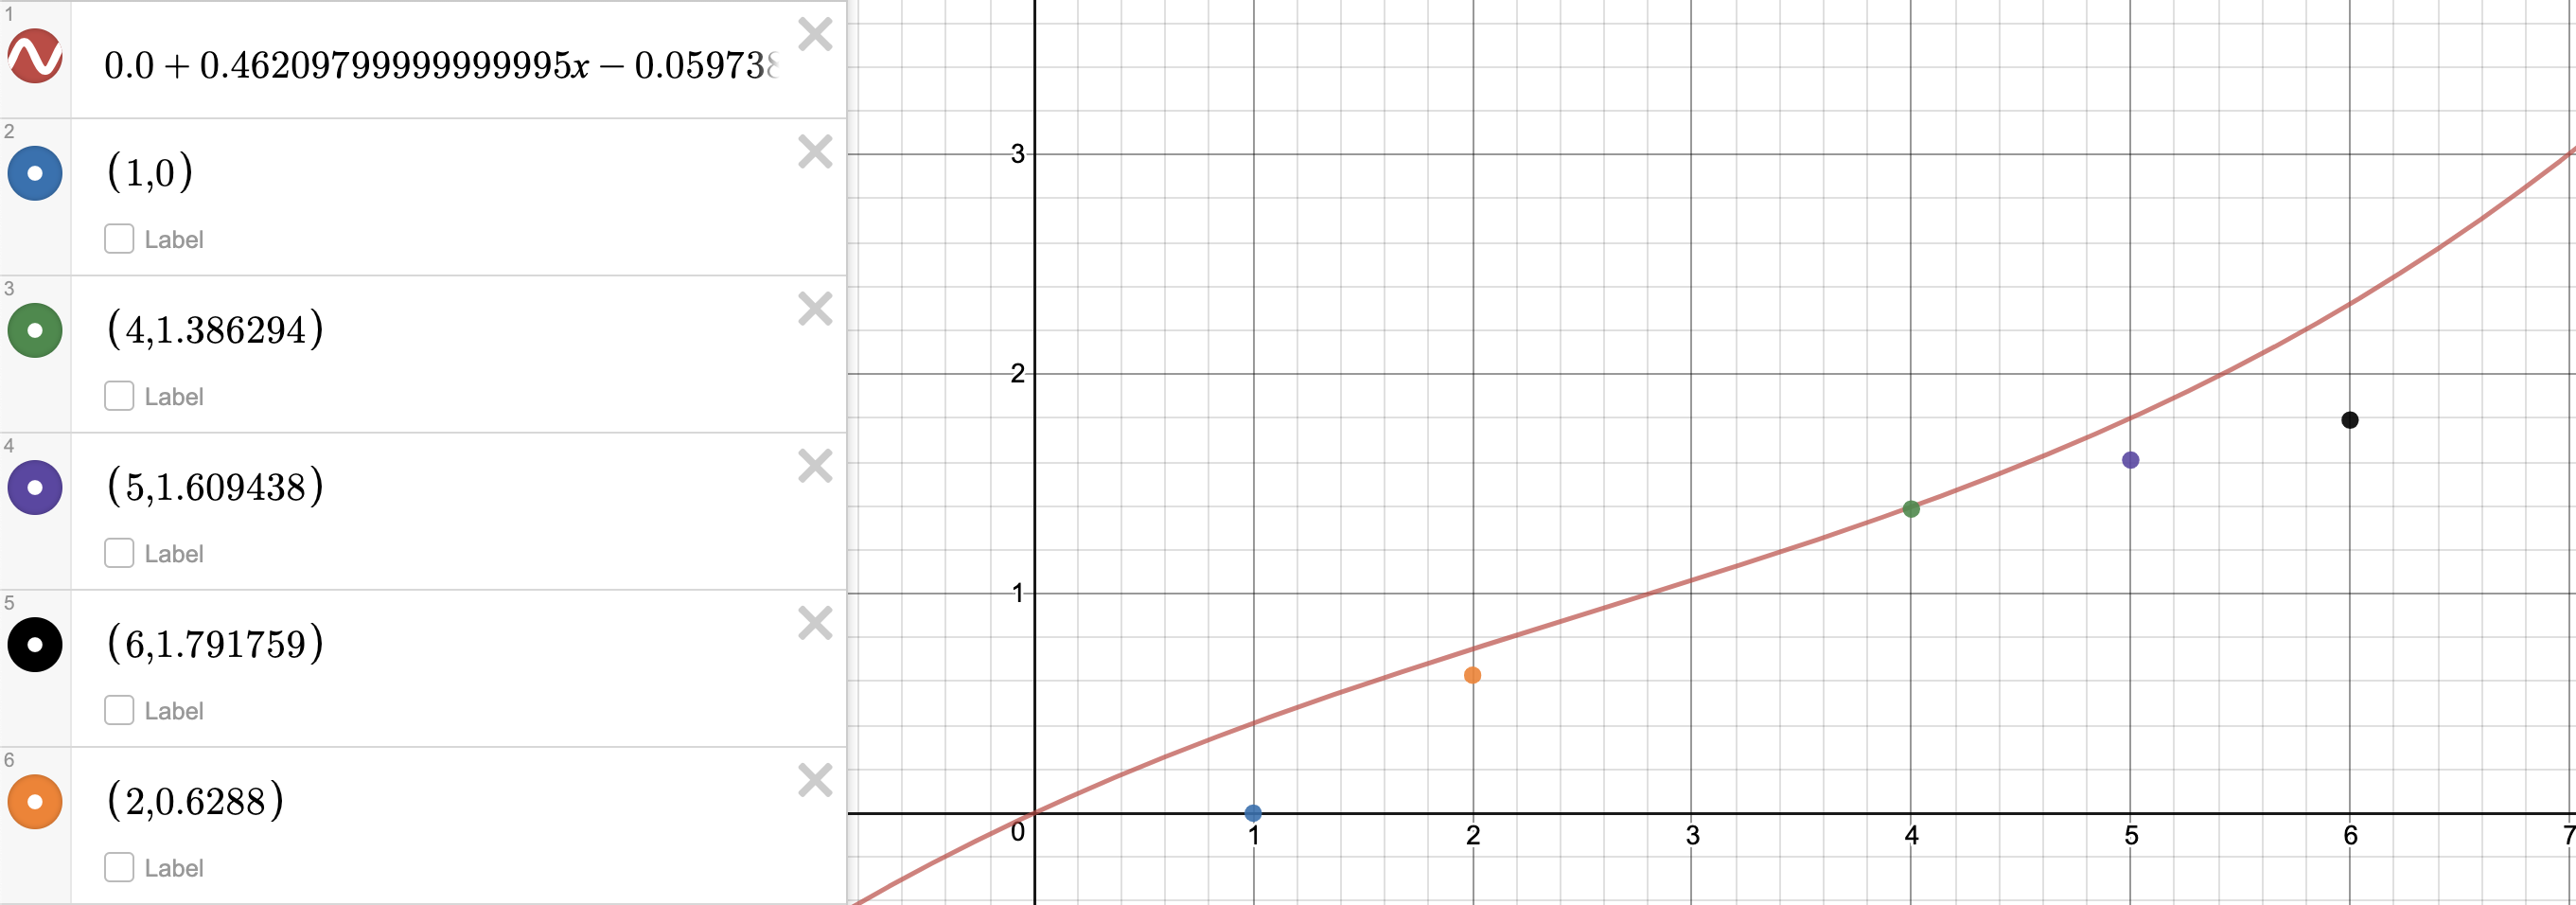
\includegraphics[width=1.0\linewidth]{plot.png}
            	\end{figure}
		
	\newpage
	\section{Appendix B}
            	\begin{figure}[h]
            		\centering
            		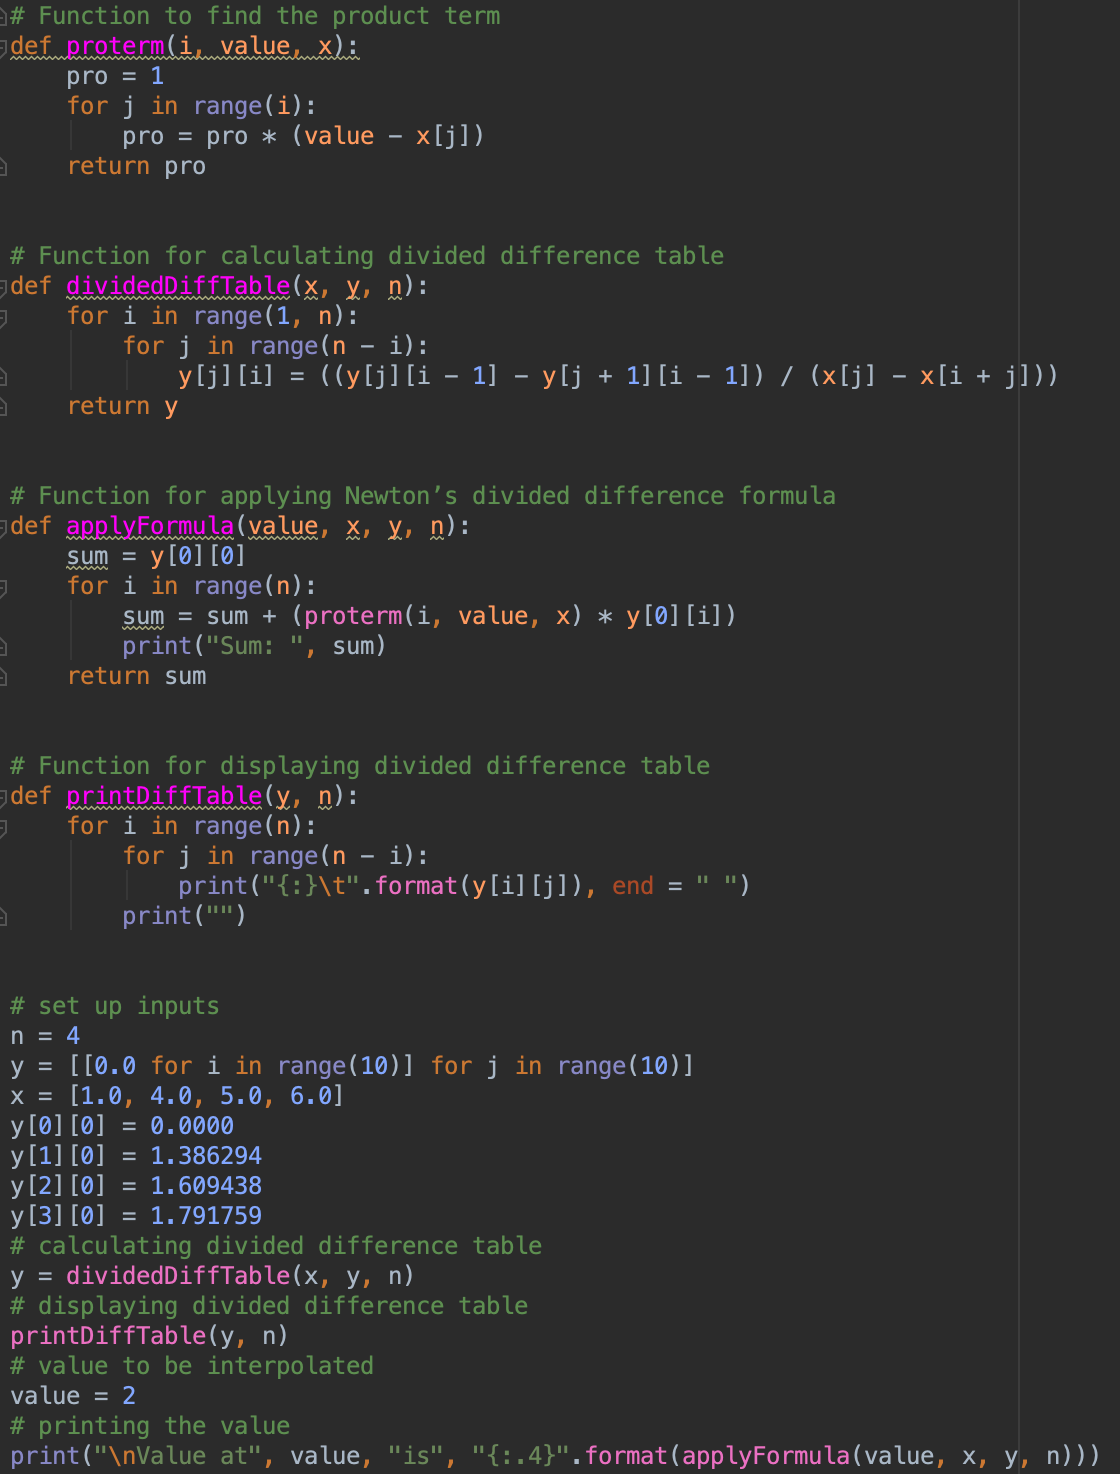
\includegraphics[width=.8\linewidth]{pythonCode.png}
            	\end{figure}
		
		
		


\end{document}
